% Modified
\documentclass{l3proj}
\usepackage{hyperref}
\usepackage{csquotes}
\usepackage{glossaries}
\usepackage{url}
\usepackage{epstopdf}
\usepackage{enumitem}

\SetBlockEnvironment{quotation}
\begin{document}
\setcounter{secnumdepth}{3}
\setcounter{tocdepth}{3}
\title{Rust DNS Server}
\author{Gordon Adam}
\date{9 February 2015}
\maketitle
\begin{abstract}

A description of rust, why it used for the dns server. why I chose this project.

\end{abstract}
\educationalconsent
\tableofcontents
%==============================================================================
\chapter{Introduction}
\label{intro}

%==============================================================================
\chapter{Research}
\label{Research}

\section{BIND}

BIND~\cite{bind} was used during the research stage in combination with Wireshark to analyse how queries should be resolved.  

\section{Teepee and rust-http}

%==============================================================================

\chapter{Planning}
\label{Planning}

After the research stage had been carried out 

\section{MoSCoW requirements}
Listed below are the project functional requirements that were identified with their priority rating based on the MoSCoW system.

\subsection{Must Have}
	\begin{itemize}[noitemsep]
	\item{ \textit{Perform iterative queries} }
	\item{ \textit{Resolve and handle resources of the type A, CNAME and SOA} }
    \item{ \textit{Implement a cache} }
    \item{ \textit{Output of Data Passing through Resolver} }
	\end{itemize}

\subsection{Should Have}
	\begin{itemize}[noitemsep]
    \item{ \textit{Commands to control the data output by the server} }
	\item{ \textit{Resolve PTR, TXT and IPv6 records} }
	\end{itemize}

\subsection{Could Have}
	\begin{itemize}[noitemsep]
	\item{ \textit{Storage of cache, that is loaded at start of server} }
	\end{itemize}

\subsection{Would Have}
	\begin{itemize}[noitemsep]
	\item{ \textit{Update of Root Servers} }
	\end{itemize}

\section{Project Timeline}

The timeline of the project was split into four main sections these sections are:
\begin{itemize}[noitemsep]
	\item{ \textit{Project Planning:} }
	\item{ \textit{Prototype Implementation:} }
	\item{ \textit{Final Implementation and Refinements:} }
	\item{ \textit{Evaluation and Testing:} }
\end{itemize}

%==============================================================================
\chapter{Design}
\label{design}

\section{User Interface}

The planned user interface for this project would be very simple, consisting of a very basic command line interface. The reason for this design choice was keep to the program as lightweight, portable and easy to use as possible. The program would also be made as intuitive as it could be, so as to cause as few problems to the end user as possible. This would involve, but not be limited to, detecting the local ip address of the users machine automatically binding to that address and informing the user of it.

There would also be a few rudimentary arguments for the user to invoke at initialisation of the server that would allow the user various options in viewing the packets crossing the server. This would involve such things as options for a full detailed output of the packets, a simplified and redacted version of the packets and an option for just the hostnames of the query in the packet and the id of the packet. Of course if no arguments were given there would be no output from the server.

The inspiration for how to display the packets on the server to the end user would be taken from the packet analyzer Wireshark, this program was heavily used during the research stage of the project. The way in which it displays the information contained in a packet is clear and informative. The way in which Wireshark displays it's output is given in ~\ref{fig:packet_output}.

\begin{figure}[h]
    \centering
    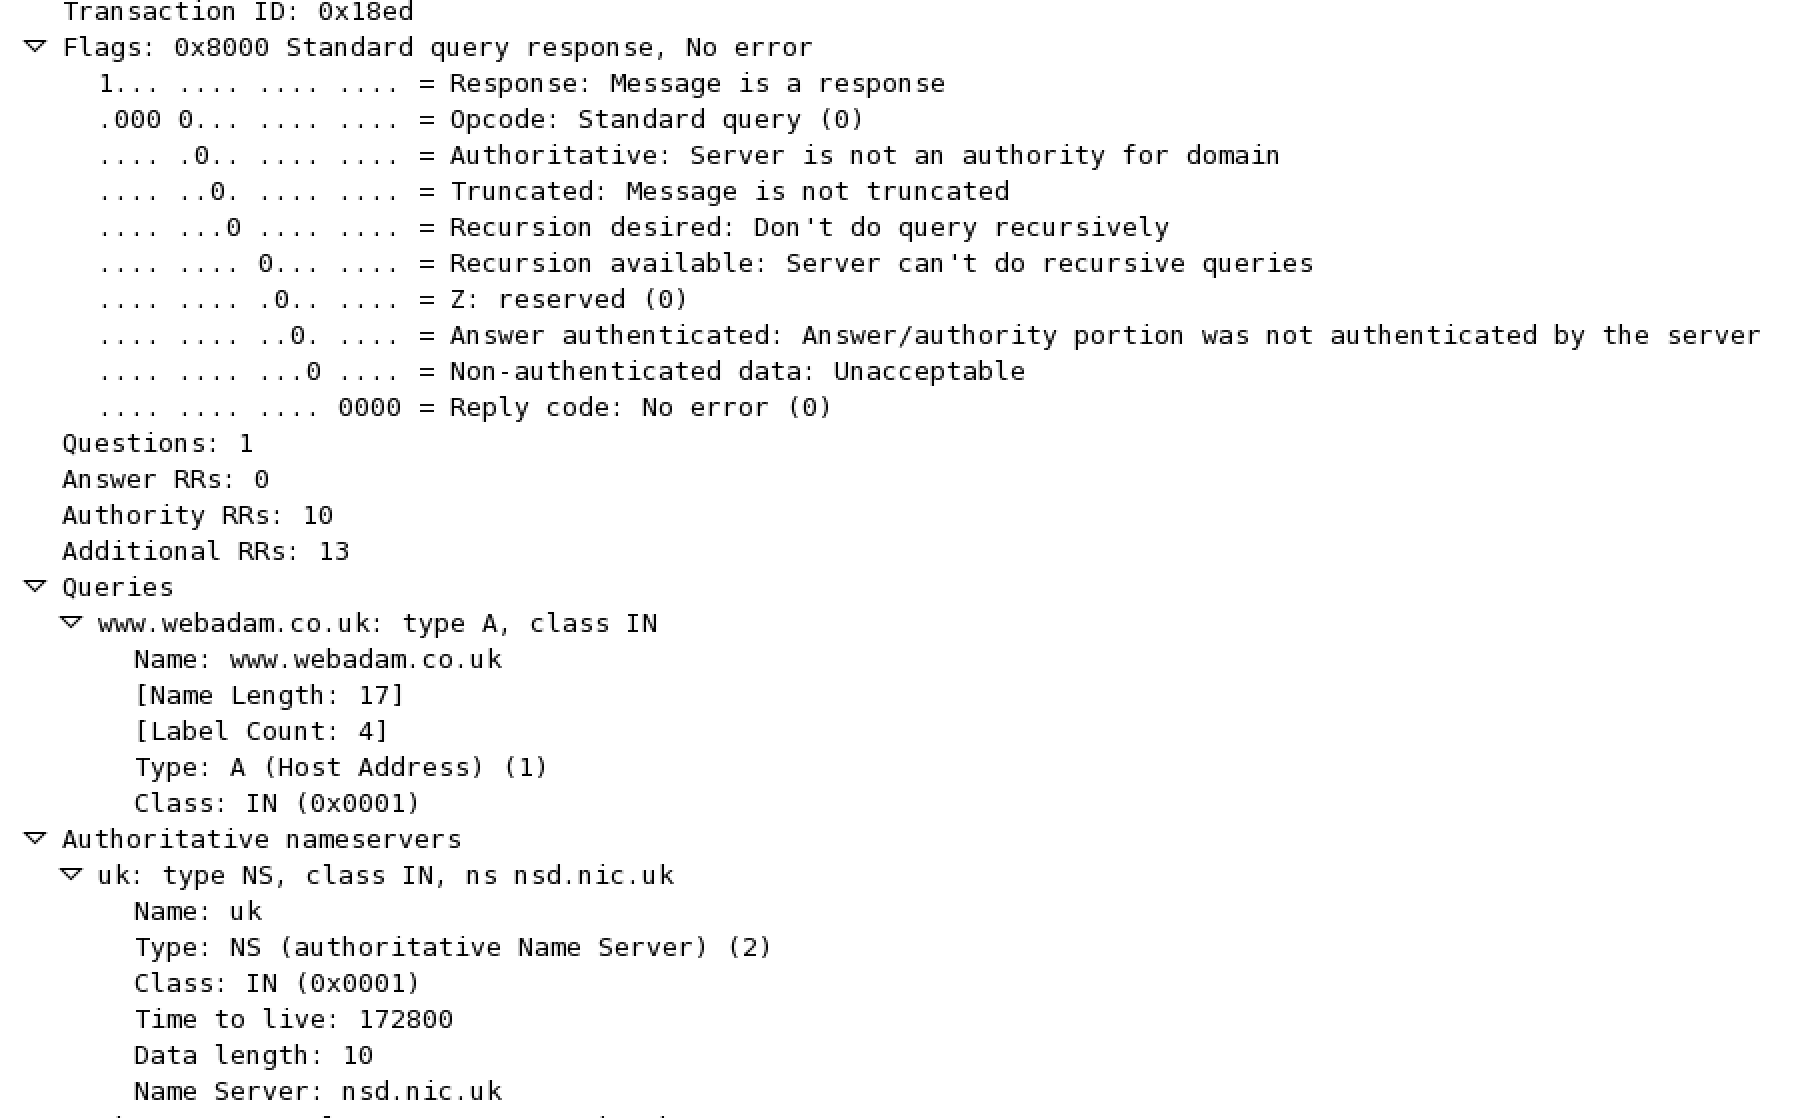
\includegraphics[width=0.7\textwidth]{images/packet_output.png}
    \caption{Wireshark Packet Output}
    \label{fig:packet_output}
\end{figure}

\section{Resolver}

The configuration for the structure of the resolver and the way in which it participates from within the domain name system has been taken largely from RFC 1035. The configuration as outlined in diagram ~\ref{figiterative} shows how the resolver achieves this. The process of querying multiple name servers to resolve a single query is called an iterative query, the specifics of this process will be covered within the implementation section. As is shown in the diagram there is also cache included. The cache is checked with each new message that comes in, to see if there is a response that matches the query. After a satisfactory response has been recieved from a name server or from within the cache it is forwarded to the client.

\begin{figure}[h]
    \centering
    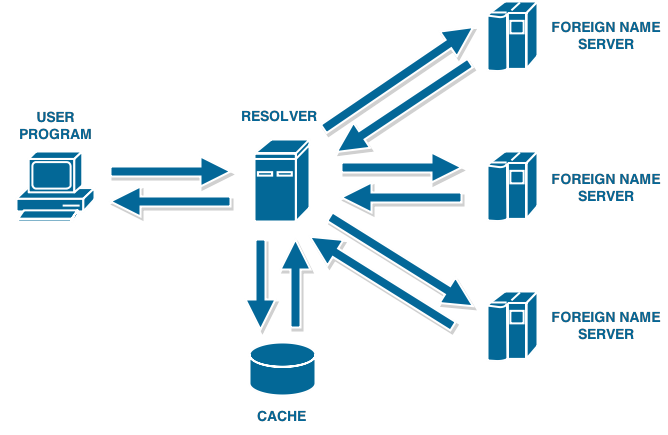
\includegraphics[width=0.6\textwidth]{images/iterative_query.png}
    \caption{Iterative Query}
    \label{fig:iterative_query}
\end{figure}

A major decision that had to be made at the time of design was which types of resources the server could handle. Ideally it should be able to support them all however with there being thirty seven seperate resource record types and a short time limit set for the development process, there would need to be priorities set on which types to support. After the research stage it was concluded that the types to be supported would be the ones most commonly witnessed through the use of Wireshark. This was done so as to reduce the chances of a resource type coming through the server that was not recognised. This led to the types A, CNAME, SOA, PTR, TXT being chosen; which stands for address record, canonical name, start of authority, pointer and text record respectively. The details of these types will be explored in section ~\ref{messageformat}.



%==============================================================================
\chapter{Implementation}
\label{impl}

\section{Message Format}
\label{messageformat}

A DNS message is split into five distinct sections, all of which will be covered within the scope of this chapter. The order of the sections contained within a message is layed out in Figure ~\ref{fig:message_format}, it is worth noting that it would not be typical for a message to contain each of the sections outlined. In fact the only mandatory field is the Header which contains details of what is contained in the rest of the message.

\begin{figure}[h]
    \centering
    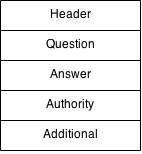
\includegraphics[width=0.25\textwidth]{images/message_format.png}
    \caption{Message Format}
    \label{fig:message_format}
\end{figure}



\subsection{Header Format}
\label{sec:header_format}

The header is the first section that is read in by the resolver and describes the content of the rest of the message. It is outlined in the following diagram.

\begin{figure}[h]
    \centering
    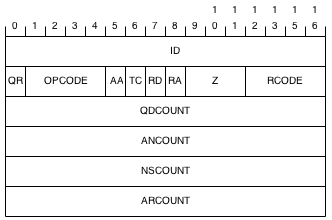
\includegraphics[width=0.5\textwidth]{images/header_format.png}
    \caption{Header Format}
    \label{fig:header_format}
\end{figure}

As can be seen in the diagram the first field is an identifier which gives a simple way to identify the message during the various stages while it is resolved. As queries come into the resolver with an identifier there is not many occasions in which one is to be generated, it is implemented however by the generation of a random number.

The next field is the QR bit which specifies whether the message is a response or a query if it is set to a '1' this identifies the message as a response and a '0' identifies it as a query. After that is the four bit opcode this specifies the type of query. As of RFC 2929~\cite{rfc2929} the various assignments for the opcodes are as follows:

\begin{description}[noitemsep]
  \item[0] Query
  \item[1] IQuery (Inverse Query)
  \item[2] Status
  \item[3] Unassigned
  \item[4] Notify
  \item[5] Update
  \item[6-15] Unassigned
\end{description}

Of these different assignments only the first on the list which is a standard query has been implemented for, otherwise the message is returned to sender with an error code.

What follows next are four single bit flags AA, TC, RD, and RA which stand for Authoritative Answer, Truncated, Recursion Desired and Recursion Available respectively. The authoritative answer flag specifies whether the answer provided in the answer section in the message is from an authority for that domain. Then next flag is truncated bit which tells you whether this message has had to be truncated during transmission. This flag never caused any trouble during implementation as truncation was handled at a lower level.

The third bit 'RD' lets the resolver know that the client desires the query to be performed recursively, support for recursive queries is optional within a name server, this is a resolver however so it is integral that recursion is supported. This means that when a message is received with the RD bit set to '1', the resolver responds to the client with the next bit 'RA' set to '1' to indicate to the client that it can handle recursive queries.

The next field is 3 bits long and is reserved for future use, it is represented by a 'Z' in figure ~\ref{fig:header_format} and should always be set to '000'. After that there is the RCODE field, this is used in a reply to indicate any errors there may be. It is represented by four bits, although it can be extended using a pseudo resource record~\cite{rfc2671}, this however is outwith the scope of this project due to time restraints. The different error codes as specified in RFC 2136~\cite{rfc2136} that may appear, excluding extensions, are:

\begin{description}[noitemsep]
	\item[0] No error condition [NOERROR]
	\item[1] Format error [FORMERR]
	\item[2] An internal server failure [SERVFAIL]
	\item[3] Name does not exist [NXDOMAIN]
	\item[4] Opcode not implemented [NOTIMP]
	\item[5] Specified operation refused [REFUSED]
	\item[6] Name that should not exist does [YXDOMAIN]
	\item[7] RRset that should not exist does [YXRRSET]
	\item[8] RRset that should exist does not [NXRRSET]
	\item[9] Not authority for zone specified [NOTAUTH]
	\item[10] Name in message not within zone specified [NOTZONE]
	\item[11-15] Unassigned
\end{description}

There was cause for a number of these error codes to be generated by the resolver within this project, the codes that have been implemented are '0', '1', '2' and '4'. The first of these '0' is obviously the simplest, this is to signify that everything is ok and there has been no problem handling the message. The next code '1' was generated and sent when there was some unspecified error while reading in a message that the resolver had received. After that was '2' this was used if the question could not be resolved due to none of the name servers responding and the request timing out. Finally '4' was simple to implement and would be called upon if an Opcode other than a query was present in the Opcode field.

The last four fields in the header are all counters and contain the number of questions, answers, authoritative name servers and additional records within the message respectively. The format of these records will be explained throughout the rest of this section.

\subsection{Question Format}

\begin{figure}[h]
    \centering
    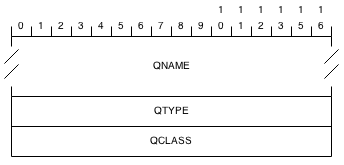
\includegraphics[width=0.5\textwidth]{images/question_format.png}
    \caption{Question Format}
    \label{fig:question_format}
\end{figure}

\subsection{Resource Record Format}

The structure of the resource record was defined in

\begin{figure}[h]
    \centering
    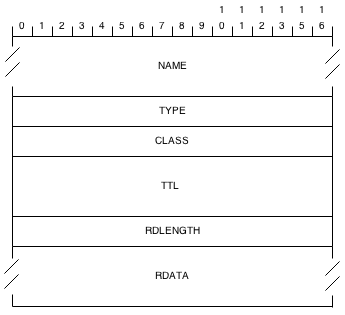
\includegraphics[width=0.5\textwidth]{images/rr_format.png}
    \caption{Resource Record Format}
    \label{fig:rr_format}
\end{figure}

\subsection{Message Compression}

There is a simple compression scheme that is used to reduce the repetition of domain names within messages. This is done by replacing the repetion of an entire, or part of a name with a pointer as demonstrated in figure ~\ref{fig:compression}. Therefore this allows a domain name to be represented by one of the following three options:

\begin{itemize}[noitemsep]
	\item{ sequence of labels ending with a 0 }
	\item{ a pointer }
	\item{ sequence of labels ending with a pointer }
\end{itemize}

\begin{figure}[h]
    \centering
    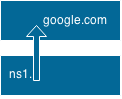
\includegraphics[width=0.3\textwidth]{images/compression.png}
    \caption{Compression}
    \label{fig:compression}
\end{figure}

A pointer is made up of two octets, the first two bits of the first octet are set to '11' this is to indicate to the DNS system that it is indeed a pointer. The next fourteen bits indicate the octet in the message at which the rest of the domain name is located. In order to implement this in the resolver an array of octets was generated from the message before reading it in. This allows the resolver to simply lookup the array of the message at the index specified whenever it encounters a pointer in order to decompress the domain name.

\subsection{Start of Authority Data Format}

\begin{figure}[h]
    \centering
    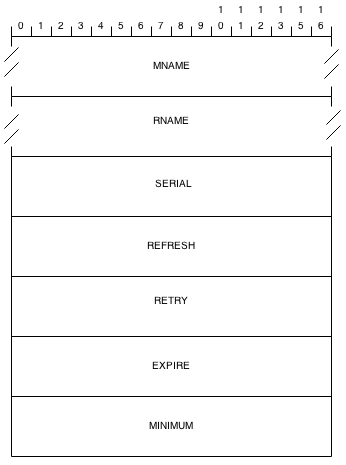
\includegraphics[width=0.5\textwidth]{images/soa_format.png}
    \caption{Start of Authority Data Format}
    \label{fig:soa_format}
\end{figure}


%==============================================================================
\chapter{Evaluation}


%==============================================================================
\chapter{Challenges}
\label{Challenges}   


%==============================================================================
\chapter{Future Work}
\label{Future Work}

%==============================================================================
\chapter{Conclusion}
\label{Conclusion}

%==============================================================================

\newpage

\bibliography{dissertation}{}
\bibliographystyle{plain}

\section{Appendices}
\subsection{Code Repositories}

\href{https://github.com/Kaffse/multi-device-audio-project}{Django Application - MDRS:}
https://github.com/Kaffse/multi-device-audio-project

\href{https://github.com/allyjweir/dissertation-teamt-tp3}{Dissertation:}
https://github.com/allyjweir/dissertation-teamt-tp3

\end{document}
